\documentclass[problem]{mcs}

\begin{pcomments}
  \pcomment{FP_directed_graphs_and_probability} %\pcomment{from: S09.cp7r}
  \pcomment{prepared in Fall'11 for the final exam by S. Dwivedi}
  \pcomment{ARM edited 12/16/11}
\end{pcomments}

\pkeywords{
  digraphs
  DAGs
  probability
}

%%%%%%%%%%%%%%%%%%%%%%%%%%%%%%%%%%%%%%%%%%%%%%%%%%%%%%%%%%%%%%%%%%%%%
% Problem starts here
%%%%%%%%%%%%%%%%%%%%%%%%%%%%%%%%%%%%%%%%%%%%%%%%%%%%%%%%%%%%%%%%%%%%%

\newcommand{\Gdir}{\overrightarrow{G}}

\begin{problem}
\bparts

\ppart For the directed acyclic graph (DAG) $G_0$ in
Figure~\ref{fig:Gdir}, a minimum-edge DAG with the same walk relation
can be obtained by removing some edges.  List these edges (use
notation $\diredge{1}{2}$ for an edge from 1 to 2):

\begin{center}
\exambox{1.5in}{0.5in}{-0.5in}
\end{center}

\begin{figure}[here]
\begin{center}
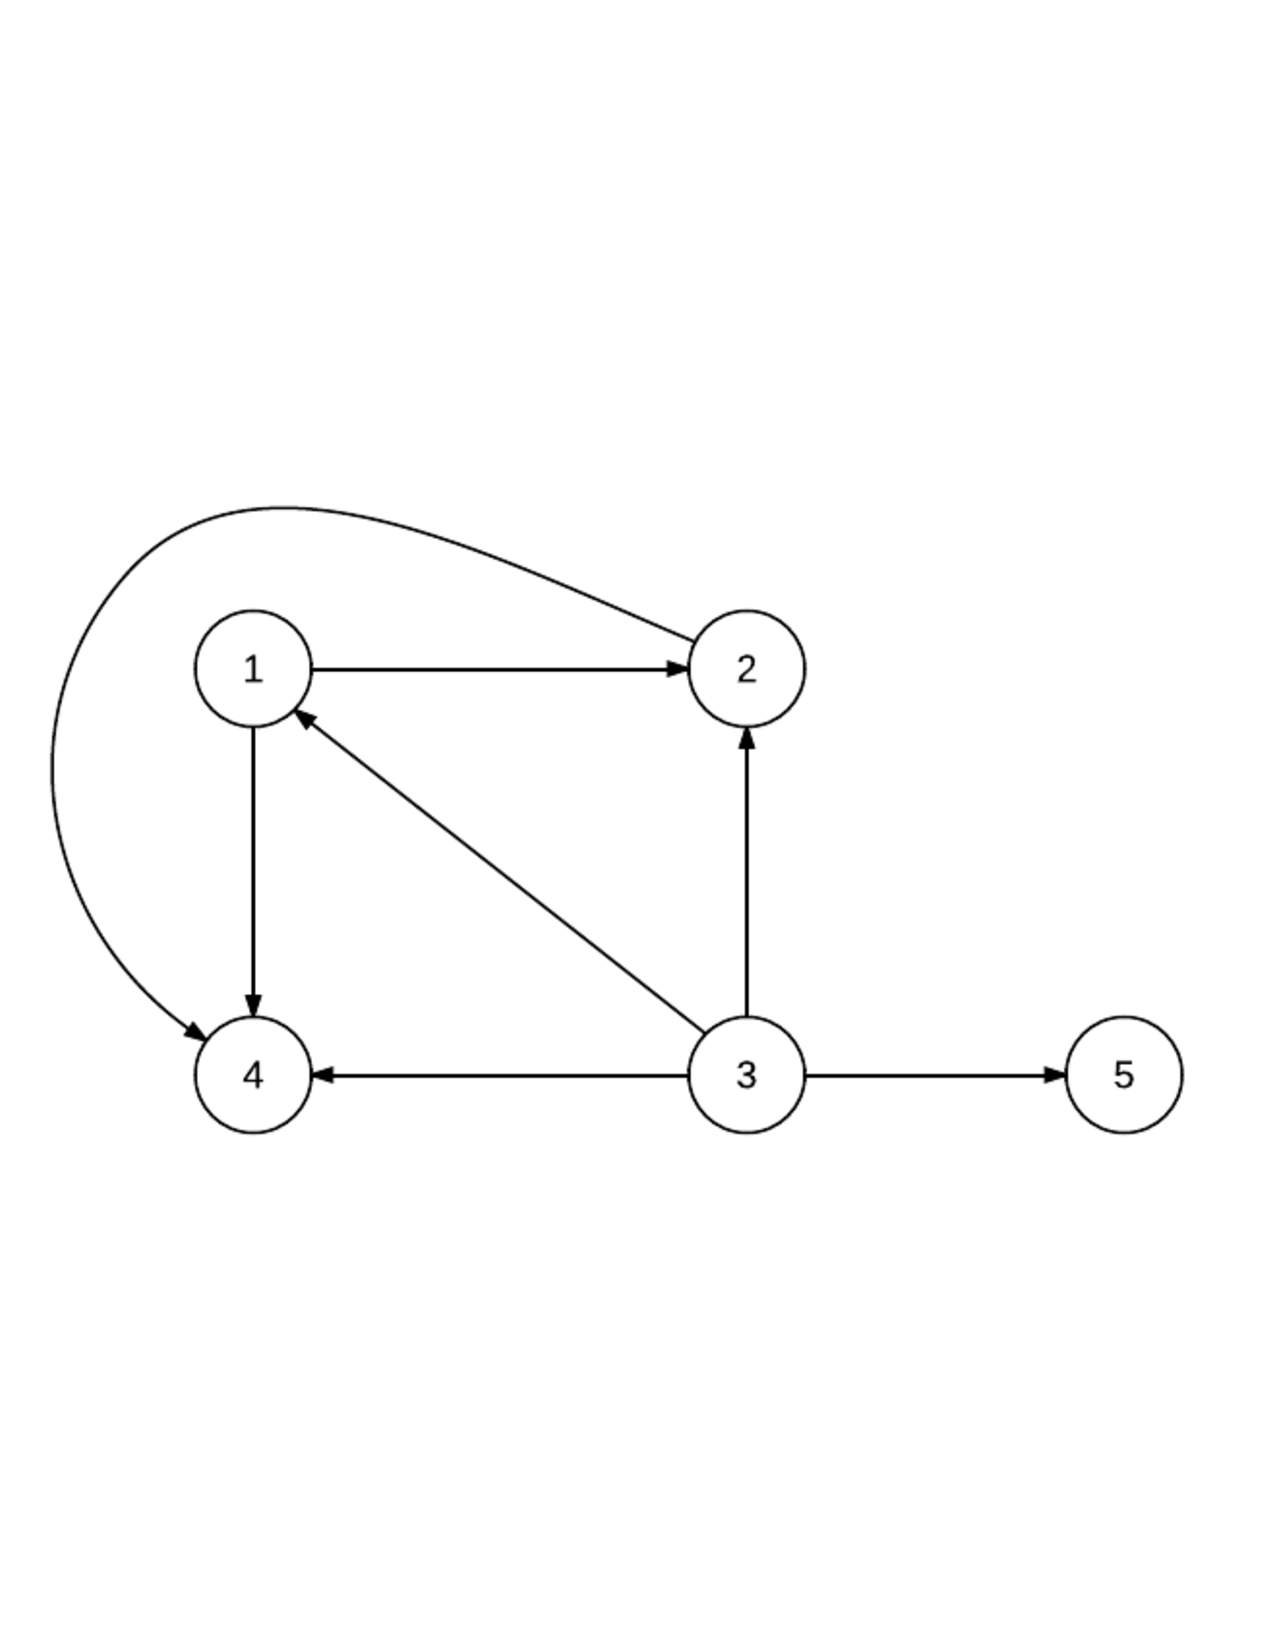
\includegraphics[width = 3.0in, height = 3.5in]{dir_graph}
\end{center}
\caption{The DAG $G_0$}
\label{fig:Gdir}
\end{figure}

\begin{solution}
After removing edges $\diredge{1}{4}$, $\diredge{3}{2}$ and $\diredge{3}{4}$, we get the
minimum DAG.
\end{solution}

\ppart List the vertices in a maximal antichain in $G_0$.

\begin{center}
\exambox{1.5in}{0.5in}{-0.3in}
\end{center}

\begin{solution}
There are multiple maximal antichains. $\set{1,5}$, $\set{2,5}$,
$\set{4,5}$, etc.
\end{solution}
\examspace[0.2in]
\eparts

\vspace{0.3in}
Let $G$ be the simple graph shown in Figure ~\ref{fig:simpleG}.

\begin{figure}[here]
\begin{center}
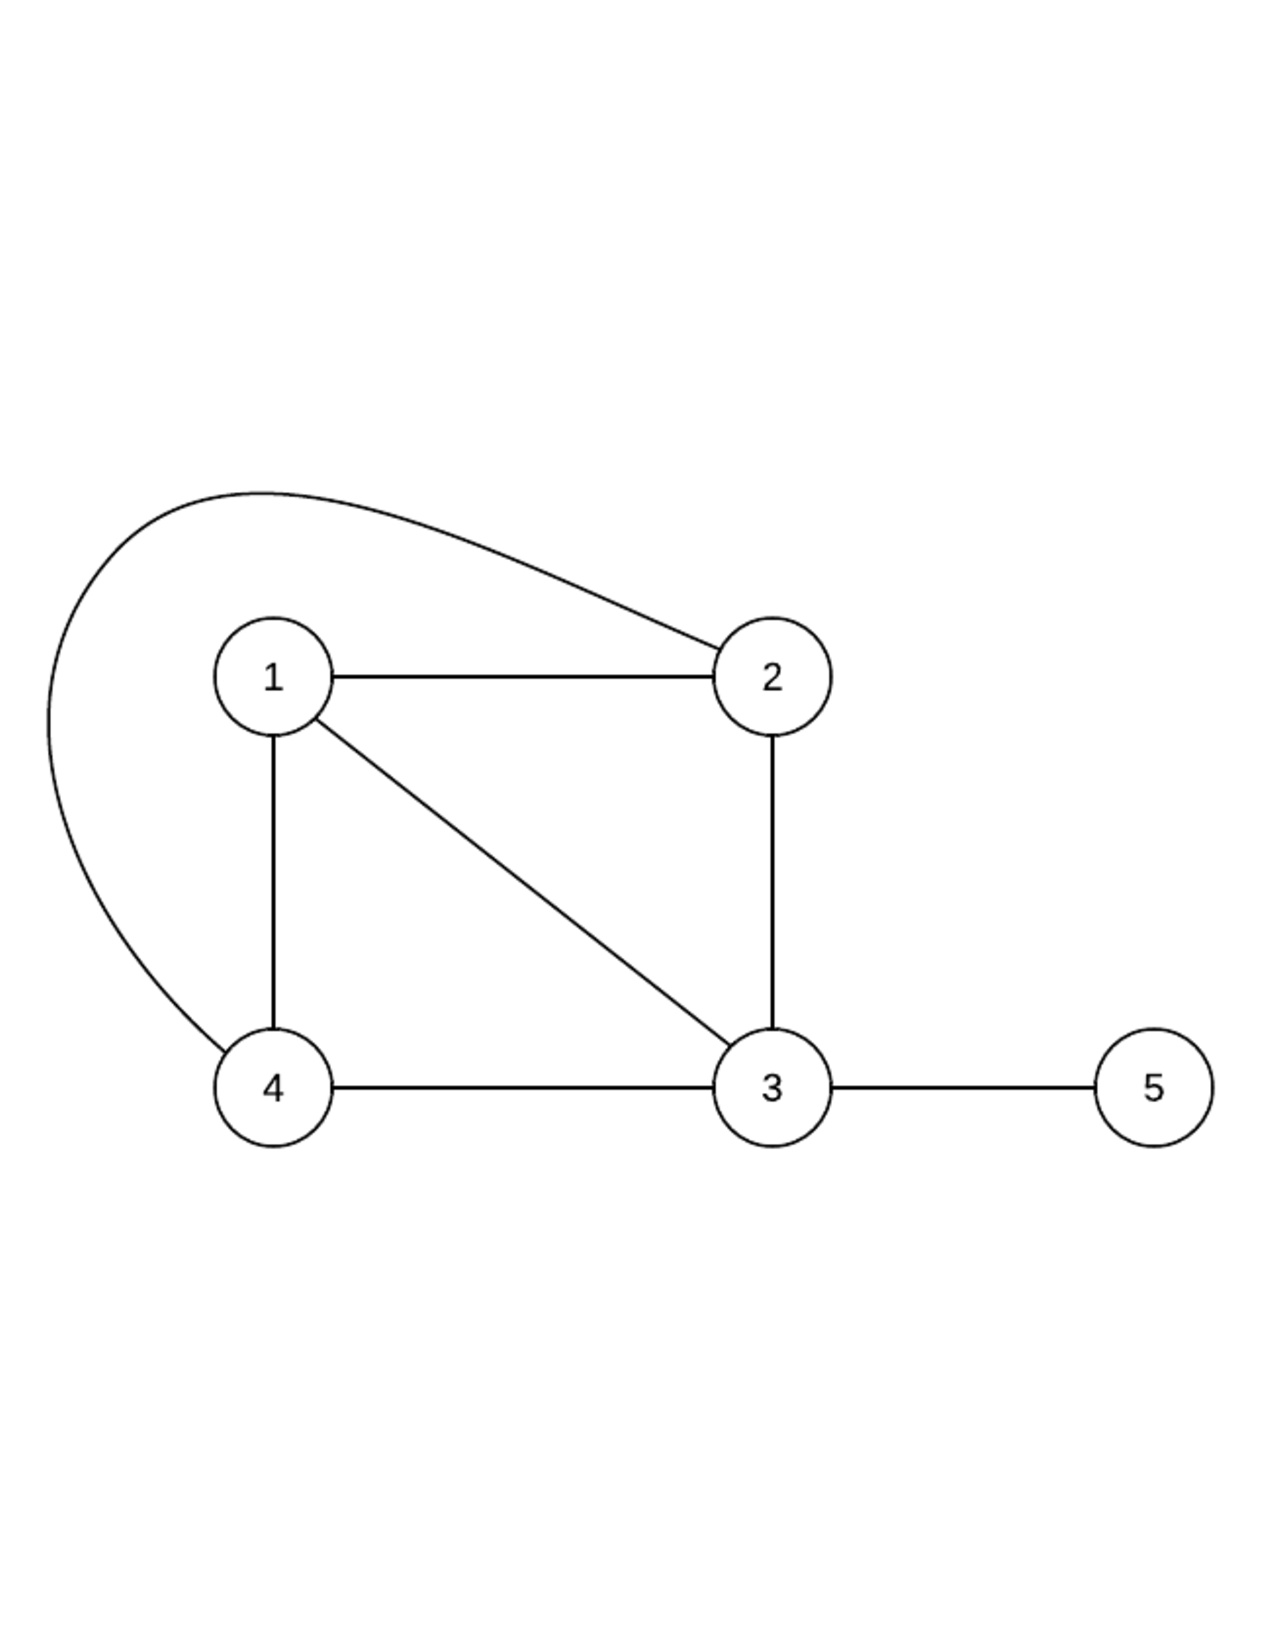
\includegraphics[width = 3.0in, height = 3.5in]{simple_graph} 
%\includegraphics[width=6in,height=7in]{mq1.jpg}
\end{center}
\caption{Simple graph $G$}
\label{fig:simpleG}
\end{figure}

A directed graph $\Gdir$ can be randomly constructed from
$G$ by assigning a direction to each edge independently with
equal likelihood.

\bparts

\ppart What is the probability that $\Gdir = G_0$?
\begin{center}
\exambox{0.5in}{0.5in}{-0.3in}
\end{center}

\begin{solution}
$2^{-\card{\edges{G}}}$
\end{solution}

\eparts

Define the following events with respect to the random graph
$\Gdir$:
\begin{align*}
T_1 \eqdef 123 \text{ is a directed cycle},\\
T_2 \eqdef 134 \text{ is a directed cycle},\\
T_3 \eqdef 124 \text{ is a directed cycle},\\
T_4 \eqdef 234 \text{ is a directed cycle}.
\end{align*}

\bparts

\ppart\label{prT1T1T2} What is
\begin{align*}
\pr{T_1}?                               & \examrule[0.75in]\\
\\
\pr{T_1 \intersect T_2}?                & \examrule[0.75in]\\
\\
\pr{T_1 \intersect T_2 \intersect T_3}? & \examrule[0.75in]
\end{align*}
\examspace[1in]

\begin{solution}
\begin{align*}
\pr{T_1} = \frac{2}{2^3} & = \frac{1}{4}\\
\pr{T_1 \intersect T_2}  & = \frac{1}{16}\\
\pr{T_1 \intersect T_2 \intersect T_3}
                        & = 0.
\end{align*}
\end{solution}

\ppart What is the probability that $\Gdir$ is a
DAG?  (You may answer with a simple numerical formula.)

\begin{center}
\exambox{4.0in}{0.5in}{-0.8in}
\end{center}

%\examspace[3in]

\begin{solution}
Using the Inclusion-Exclusion principle,

\begin{align*}
\pr{\Gdir \text{ is a DAG}}
   & = 1 - \pr{T_1 \union T_2 \union T_3 \union T_4}\\
   & = 1 - \sum_{i=1}^{4} \pr{T_i} + \sum_{i\neq j} \pr{T_i \intersect T_j}\\
   & \quad - \sum_{i\neq j \neq k} \pr{T_i \intersect T_j \intersect T_k}
        + \pr{T_1 \intersect T_2 \intersect T_3 \intersect T_4}\\
   & = 1 - 4 \cdot \frac{1}{4} + 6 \cdot \frac{1}{16} - 0 + 0\\
   & = \frac{3}{8}
\end{align*}


Here we're using the obvious fact that the results of
part~\eqref{prT1T1T2} for $T_1,T_2,T_3$ hold for $T_i,T_j,T_k$ for all
distinct values of $i,j,k \in [1,4]$.

\end{solution}

\eparts

\end{problem}

%%%%%%%%%%%%%%%%%%%%%%%%%%%%%%%%%%%%%%%%%%%%%%%%%%%%%%%%%%%%%%%%%%%%%
% Problem ends here
%%%%%%%%%%%%%%%%%%%%%%%%%%%%%%%%%%%%%%%%%%%%%%%%%%%%%%%%%%%%%%%%%%%%%

\endinput
